% Source code by Nguyễn Văn Lộc
\documentclass[a4paper]{article}
\usepackage[fontsize=13pt]{scrextend}
\usepackage[utf8]{vietnam}
\usepackage{amsmath}
\usepackage{amsfonts}
\usepackage{algorithm}
\usepackage[noend]{algpseudocode}
% Credit: fit@hcmus template
\makeatletter
\def\BState{\State\hskip-\ALG@thistlm}
\makeatother
\usepackage{caption}
\usepackage{ragged2e}
\usepackage{chngcntr}
\usepackage{xcolor}
\usepackage{colortbl}
\usepackage{titlesec}
\usepackage{mdframed}
\usepackage{amssymb}
\usepackage{pgf,tikz,pgfplots}
\usepackage{graphicx}
\graphicspath{ {figures/} }
\usepackage{array}
\usepackage{cases}
\usepackage{listings}
\usepackage{tabulary}
\usepackage{color}
\usepackage{float} 
\usepackage{hyperref}
\usepackage{multirow}
\usepackage{minitoc}
\pgfplotsset{compat=1.5}
\usepackage{mathrsfs}
\usetikzlibrary{arrows, calc}
\usepackage{fancyhdr}
\usepackage{longtable}
\usepackage{verbatim}
\usepackage{indentfirst}
\usepackage{minted}
\usepackage{enumitem}
\usepackage[
backend=bibtex,
style=numeric,
natbib=true,
url=true, 
doi=true,
eprint=false,
sorting=nyt
]{biblatex}
\addbibresource{refs.bib}
\pagestyle{fancy}
\pagestyle{empty}
\definecolor{dkgreen}{rgb}{0,0.6,0}
\definecolor{gray}{rgb}{0.5,0.5,0.5}
\definecolor{mauve}{rgb}{0.58,0,0.82}
\lstset{frame=tb,
  language=Python,
  aboveskip=3mm,
  belowskip=3mm,
  showstringspaces=false,
  columns=flexible,
  basicstyle={\small\ttfamily},
  numbers=none,
  numberstyle=\tiny\color{gray},
  keywordstyle=\color{blue},
  commentstyle=\color{dkgreen},
  stringstyle=\color{mauve},
  breaklines=true,
  breakatwhitespace=true,
  tabsize=3
}
\hypersetup{
  colorlinks=true,
  linkcolor=blue,
  filecolor=magenta,      
  urlcolor=red,
  pdftitle={xv6 Lab 01},
  % pdfpagemode=FullScreen,
}
\newcommand{\tabitem}{~~\llap{\textbullet}~~}
\usepackage[left=2cm,right=2cm,top=2cm,bottom=2cm]{geometry}
\author{Hồ Minh Quang}
\newmdenv[linecolor=black,skipabove=\topsep,skipbelow=\topsep,
leftmargin=-5pt,rightmargin=-5pt,
innerleftmargin=5pt,innerrightmargin=5pt]{mybox}
\fancyhf{}
\lhead{Báo cáo bài tập: xv6 và Unix}
\chead{}
\rhead{}
\cfoot{\hspace{4.65cm} \thepage}
\rfoot{}
\lfoot{}
\pagestyle{fancy}
\renewcommand{\headrulewidth}{0pt}
\renewcommand{\footrulewidth}{0pt}
\begin{document}
  \begin{titlepage}
	\begin{mybox}
		\begin{center}
			\fontsize{12}{12}\selectfont
			\textbf{ĐẠI HỌC QUỐC GIA THÀNH PHỐ HỒ CHÍ MINH}\\
			\textbf{TRƯỜNG ĐẠI HỌC KHOA HỌC TỰ NHIÊN}\\
			\textbf{KHOA CÔNG NGHỆ THÔNG TIN}
		\end{center}
		\vskip 1.5 cm
		\begin{figure}[H]
			\begin{center}
				
\includegraphics[scale=0.5]{figures/fit-logo-chuan-V3}
				\captionlistentry{Logo khoa Công nghệ thông tin}
				\label{fig:fit-logo}
			\end{center}
		\end{figure}
		\vskip 1 cm
		\begin{center}
			\fontsize{16}{12}\selectfont
			\textbf{Hồ Minh Quang - Lê Hoàng Sơn}
			\vskip 0.75cm
			\textbf{BÁO CÁO BÀI TẬP}\\
			\fontsize{24}{20}\selectfont
			\textbf{HỆ ĐIỀU HÀNH}\\
			\fontsize{16}{12}\selectfont
			\textbf{xv6 và Unix}
		\end{center}
		\vskip 10 cm
		\begin{center}
			\textbf{THÀNH PHỐ HỒ CHÍ MINH, THÁNG 10 NĂM 2024}
		\end{center}
	\end{mybox}
	
	\pagebreak
	\thispagestyle{empty}
	
	\begin{mybox}
		\begin{center}
			\fontsize{12}{12}\selectfont
			\textbf{ĐẠI HỌC QUỐC GIA THÀNH PHỐ HỒ CHÍ MINH}\\
			\textbf{TRƯỜNG ĐẠI HỌC KHOA HỌC TỰ NHIÊN}\\
			\textbf{KHOA CÔNG NGHỆ THÔNG TIN}
		\end{center}
		\vskip 1.5 cm
		\begin{figure}[H]
			\begin{center}
				
\includegraphics[scale=0.5]{figures/fit-logo-chuan-V3}
			\end{center}
		\end{figure}
		\vskip 1 cm
		\begin{center}
			\fontsize{16}{12}\selectfont
			\textbf{BÁO CÁO BÀI TẬP}\\
			\fontsize{24}{20}\selectfont
			\textbf{HỆ ĐIỀU HÀNH}\\
			\fontsize{16}{12}\selectfont
			\textbf{xv6 và Unix}
		\end{center}
		\vskip 4 cm
		\fontsize{14}{12}\selectfont
		\textbf{Môn học:} Hệ điều hành\\
		\textbf{Mã môn học:} CSC10007\\
		\textbf{Các sinh viên tham gia:} Hồ Minh Quang - 22120295; Lê Hoàng Sơn - 22120311\\
		\textbf{Lớp:} 22\_4\\
		\vskip 5 cm
		\begin{center}
			\textbf{THÀNH PHỐ HỒ CHÍ MINH, THÁNG 10 NĂM 2024}
		\end{center}
	\end{mybox}
\end{titlepage}
  \newpage
  
  \tableofcontents
  \renewcommand{\listfigurename}{Danh sách hình}
  \listoffigures
%  \listoftables
  \newpage
  \nopagebreak
  \counterwithin{figure}{section}
  \setcounter{secnumdepth}{2}
\section{Bảng phân công công việc và cài đặt xv6}
\subsection{Bảng phân công công việc}
Dưới đây là bảng phân công công việc của nhóm:

\centering
\vskip 0.25 cm
\begin{tabular}{|c|c|c|}
	\hline
	Họ và tên & Chức năng đảm nhiệm & Tiến độ hoàn thành\\
	\hline
	Hồ Minh Quang & Lệnh \textbf{pingpong} & 100\%\\
	\hline
	Hồ Minh Quang & Lệnh \textbf{xargs} & 100\%\\
	\hline
	Lê Hoàng Sơn & Lệnh \textbf{primes} & 100\%\\
	\hline
	Lê Hoàng Sơn & Lệnh \textbf{find} & 100\%\\
	\hline
	Hồ Minh Quang & Viết báo cáo cho các lệnh & 100\%\\
	Lê Hoàng Sơn & được đảm nhiệm & 100\%\\
	\hline
\end{tabular}

\justifying
\subsection{Cài đặt xv6}
Các hướng dẫn cài đặt xv6 đã có sẵn trên Lab 6.1810 của MIT \cite{mit-xv6}. Dưới đây là kết quả cài đặt xv6 của nhóm:

\begin{figure}[h!]
	\centering
	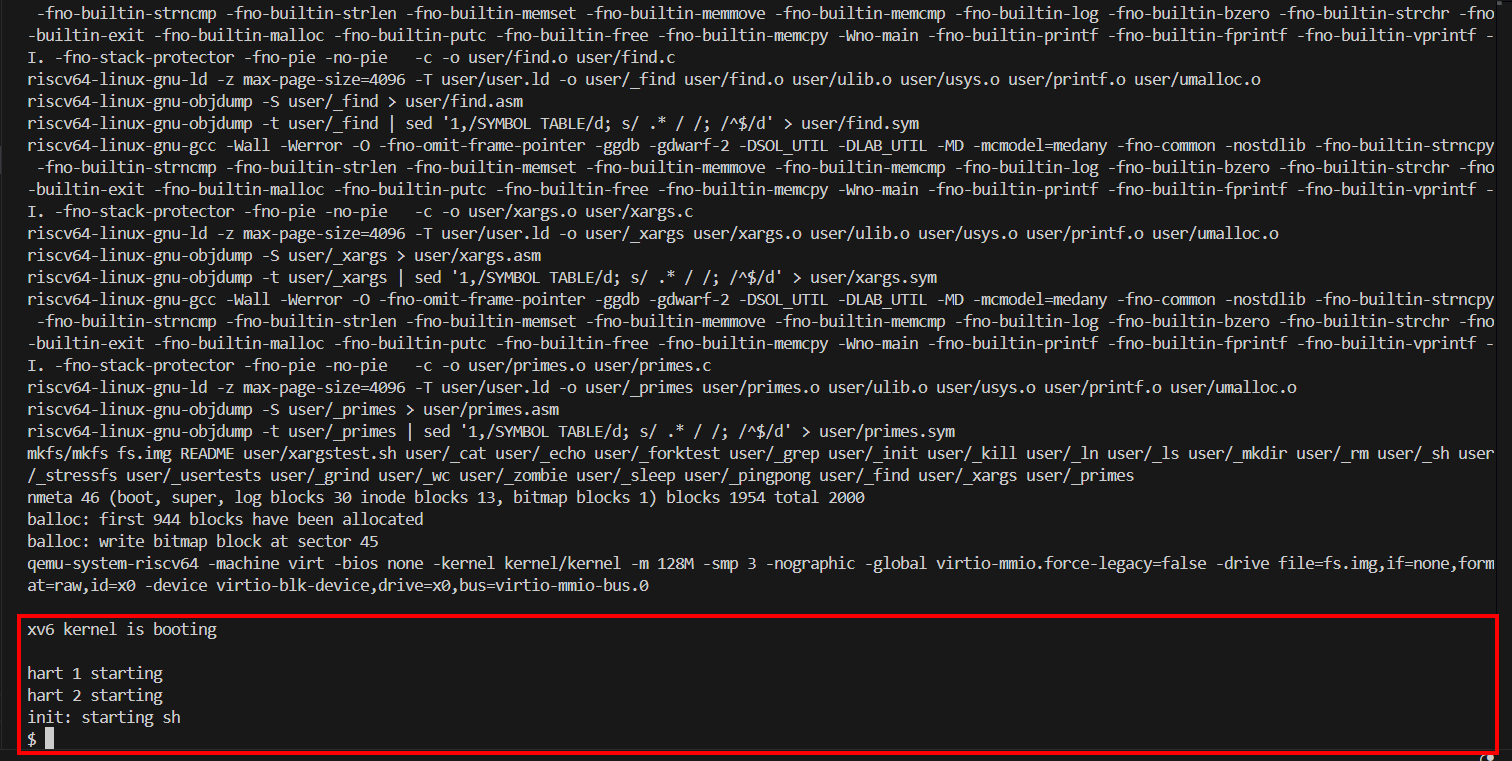
\includegraphics[width=0.9\textwidth]{figures/xv6-launch}
	\caption{Khởi động xv6 trên Linux}
\end{figure}

\justifying
Lệnh \mintinline{shell}|$ git diff origin -- . > 22120295_22120311.patch| được dùng để tạo \linebreak bản vá \verb|diff|.

\subsection{Một số hàm có sẵn trong mã nguồn}
\underline{\mintinline{C++}|int read(int _fd, void* _buffer, int _nbytes)|:} Hàm này được dùng để đọc một số lượng byte trong tập tin \verb|_fd| và lưu vào vùng nhớ con trỏ \verb|_buffer| trỏ tới.

\underline{\mintinline{C++}|int write(int _fd, void* _buffer, int _nbytes)|:} Hàm này được dùng để ghi một số lượng byte vào tập tin \verb|_fd| từ vùng nhớ con trỏ \verb|_buffer| trỏ tới.
  \section{Các lệnh đã thiết lập}
\subsection{Lệnh sleep}
\underline{\textbf{Chức năng của lệnh:}} Lệnh \verb|sleep <number of ticks>| cho phép người dùng dừng hệ thống trong số ticks nhất định (\textbf{ticks} là một đơn vị thời gian được quy định trong hệ điều hành xv6) \cite{mit-xv6}.

\underline{\textbf{Thiết lập thuật toán:}} Gọi hàm \verb|sleep| từ thư viện \verb|user.h| được cung cấp sẵn trong xv6 và chuyển chuỗi số trong câu lệnh về kiểu số nguyên. Lệnh sẽ báo lỗi khi nhập sai cú pháp.

Dưới đây là kết quả chạy thử trên \verb|qemu| và kiểm tra lệnh \verb|sleep| bằng chương trình kiểm thử:
\begin{figure}[htp!]
	\centering
	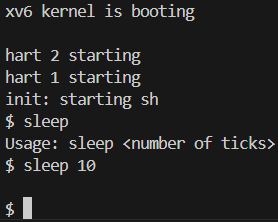
\includegraphics[width=0.5\textwidth]{figures/exec-sleep}
	\caption{Kết quả chạy thử \textbf{sleep} trên \textbf{qemu}}
\end{figure}
\begin{figure}[htp!]
	\centering
	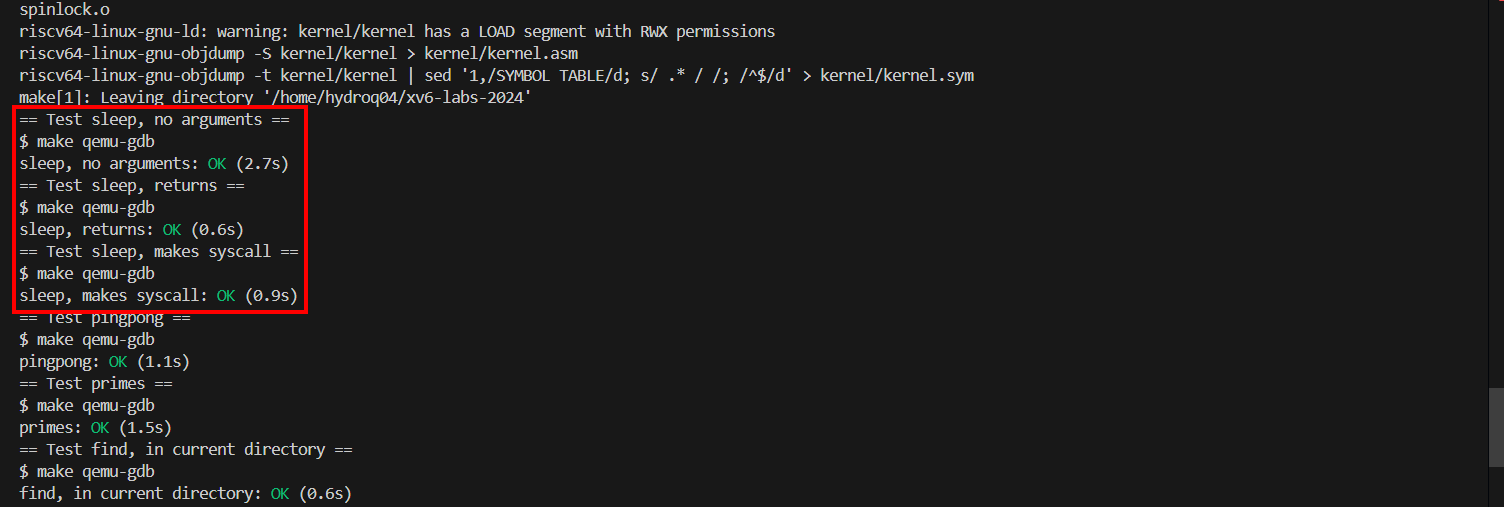
\includegraphics[width=0.9\textwidth]{figures/sleep-test}
	\caption{Kết quả kiểm thử \textbf{sleep} bằng công cụ chấm bài \textbf{grade} của MIT}
\end{figure}

\newpage
  \subsection{Lệnh pingpong}
\underline{\textbf{Chức năng của lệnh:}} Lệnh \verb|pingpong| thực hiện việc truyền 1 byte dữ liệu giữa hai tiến trình bằng một cặp \textbf{pipe} (\textbf{pipe} là một đường dẫn dữ liệu giữa hai tiến trình, với một đầu được cố định để đọc dữ liệu từ thiết bị nhập và đầu còn lại ghi dữ liệu ra \linebreak thiết bị xuất) \cite{mit-xv6}.

\underline{\textbf{Thiết lập thuật toán:}}
\begin{enumerate}[labelindent=1em, labelsep=0.2cm, leftmargin=1cm, wide=\parindent, topsep=0.1cm, itemsep=-1ex, partopsep=1.5ex, parsep=1.5ex]
	\item Khởi tạo hai \textbf{pipe} \verb|p_in| và \verb|p_out| và phân chia tiến trình ra làm hai bằng hàm \verb|fork()|. Tiến trình con (\verb|fork() == 0|) dùng \verb|p_in| để đọc dữ liệu và truyền qua tiến trình cha. Tiến trình cha (\verb|fork() > 0|) dùng \verb|p_out| làm điều tương tự với tiến trình con.
	\item Tiến trình con truyền 1 byte dữ liệu (trong mã nguồn dùng chữ \verb|'i'|) cho tiến trình cha. Tiến trình cha sau khi nhận được thì in số thứ tự của nó và thông báo \verb|received ping|.
	\item Tiến trình cha truyền 1 byte dữ liệu (trong mã nguồn dùng chữ \verb|'o'|) cho tiến trình con. Tiến trình con sau khi nhận được thì in số thứ tự của nó và thông báo \verb|received pong|.
\end{enumerate}

Lệnh sẽ báo lỗi khi người dùng nhập sai cú pháp.

Dưới đây là kết quả chạy thử trên \verb|qemu| và kiểm tra lệnh \verb|pingpong| bằng chương trình kiểm thử:
\begin{figure}[htp!]
	\centering
	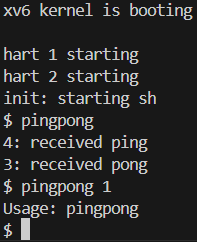
\includegraphics[width=0.5\textwidth]{figures/exec-pingpong}
	\caption{Kết quả chạy thử \textbf{pingpong} trên \textbf{qemu}}
\end{figure}
\begin{figure}[htp!]
	\centering
	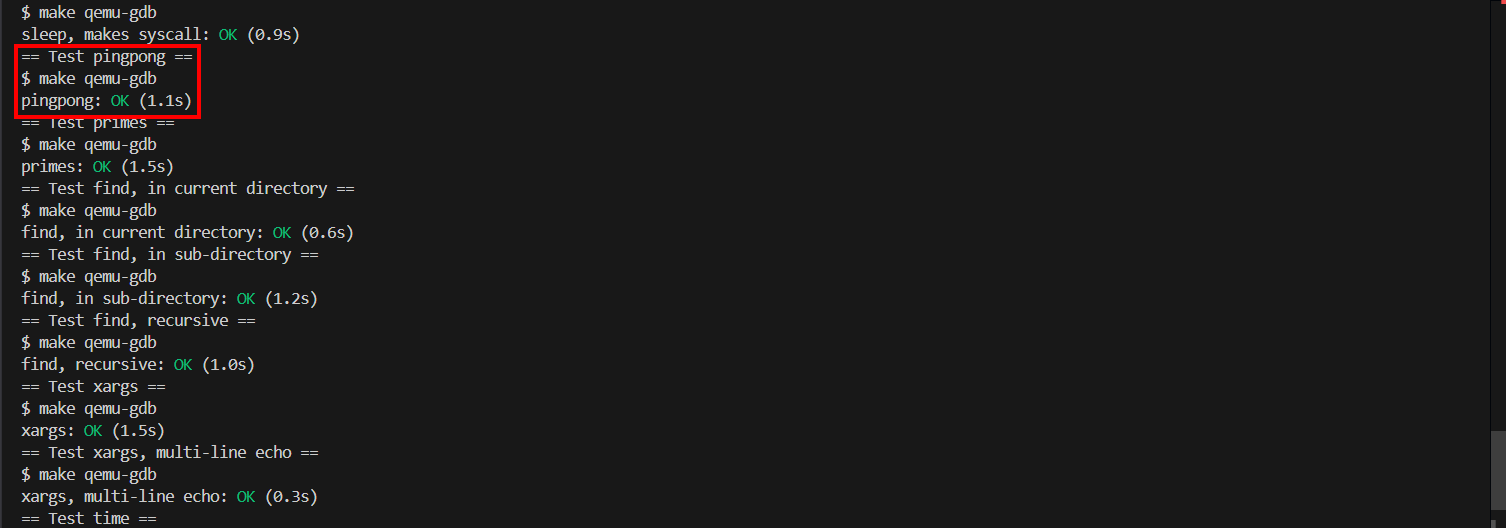
\includegraphics[width=0.9\textwidth]{figures/pingpong-test}
	\caption{Kết quả kiểm thử \textbf{pingpong} bằng công cụ chấm bài \textbf{grade} của MIT}
\end{figure}
  \subsection{Lệnh primes}
\underline{\textbf{Chức năng của lệnh:}} Lệnh \verb|primes| in ra các số nguyên tố từ 2 đến 280 qua phương pháp sàng Eratosthenes \cite{mit-xv6} \cite{primes}.

\textbf{Phương pháp sàng Eratosthenes:}
\begin{enumerate}[labelindent=1em, labelsep=0.2cm, leftmargin=1cm, wide=\parindent, topsep=0.1cm, itemsep=-1ex, partopsep=1.5ex, parsep=1.5ex]
	\item Lập danh sách các số tự nhiên từ 2 đến $n$.
	\item Đánh dấu số đầu tiên (đặt là $a$) chưa bị gạch bỏ trong danh sách là số nguyên tố.
	\item Loại bỏ các số là bội của $a$. Lặp lại từ bước 2 cho đến khi không còn đánh dấu được số nào nữa.
\end{enumerate}

\begin{figure}[htp!]
	\centering
	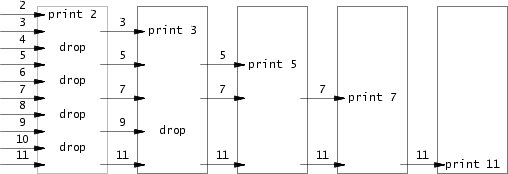
\includegraphics[width=0.9\textwidth]{figures/Eratosthenes-sieve}
	\caption{Hình minh họa thuật toán sàng Eratosthenes}
\end{figure}

\underline{\textbf{Thiết lập thuật toán:}}

Hàm \mintinline{C++}|void primes(int pL)|:
\begin{enumerate}[labelindent=1em, labelsep=0.2cm, leftmargin=1cm, wide=\parindent, topsep=0.1cm, itemsep=-1ex, partopsep=1.5ex, parsep=1.5ex]
	\item Đọc số đầu tiên trong đường dẫn \verb|pL| (\verb|pL| là một đường dẫn đã được thiết lập trước, chứa các số chưa được đánh dấu/chưa bị loại bỏ khỏi danh sách). Nếu không đọc được số nào thì kết thúc hàm, ngược lại thì in số đó ra màn hình.
	\item Thiết lập một đường dẫn (pipe) dùng để lưu các số chưa được đánh dấu/chưa bị loại bỏ khỏi danh sách.
	\item Phân chia tiến trình ra làm hai. Tiến trình cha xử lý việc loại bỏ các số là bội của số đầu tiên, trong khi tiến trình con thì gọi đệ quy hàm \verb|primes|.
\end{enumerate}

Lệnh sẽ báo lỗi khi người dùng nhập sai cú pháp.

\underline{\textbf{Khó khăn đã gặp phải:}}
\begin{itemize}[labelindent=1em, labelsep=0.2cm, leftmargin=1cm, wide=\parindent, topsep=0.1cm, itemsep=-1ex, partopsep=1.5ex, parsep=1.5ex]
	\item Hiểu và xử lí được cách dãy số được truyền qua lại giữa các tiến trình.
	\item Vì tài nguyên của xv6 có hạn, nên các mô tả tệp sẽ phải đóng ngay và được đóng một cách hợp lí để tránh ảnh hưởng tới quá trình xử lí.
\end{itemize}

Dưới đây là kết quả kiểm tra lệnh \verb|primes| bằng chương trình kiểm thử:
\begin{figure}[htp!]
	\centering
	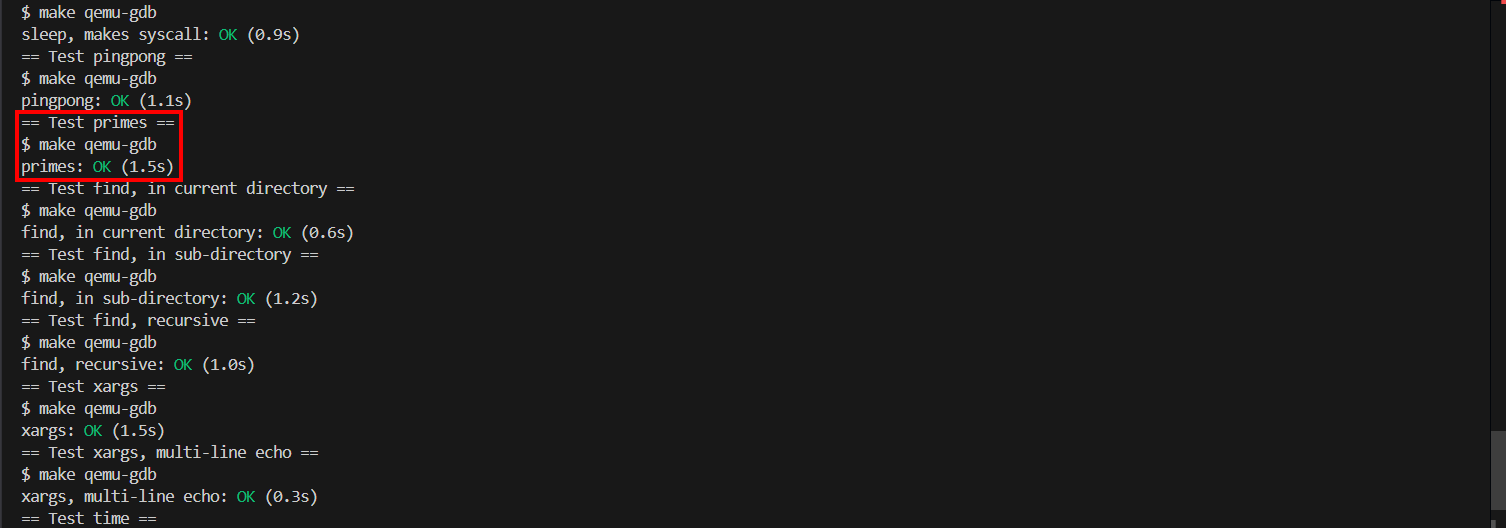
\includegraphics[width=0.9\textwidth]{figures/primes-test}
	\caption{Kết quả kiểm thử \textbf{primes} bằng công cụ chấm bài \textbf{grade} của MIT}
\end{figure}
  \subsection{Lệnh find}
\underline{\textbf{Chức năng của lệnh:}} Lệnh \verb|find <dir> <fname1> [fname2] ...| được dùng để tìm kiếm các tập tin tên \verb|fname1|, \verb|fname2|... trong thư mục \verb|dir| \cite{mit-xv6}.

\underline{\textbf{Thiết lập thuật toán:}}

Hàm \mintinline{C++}|void find(char* root, char* name)|:
\begin{enumerate}[labelindent=1em, labelsep=0.2cm, leftmargin=1cm, wide=\parindent, topsep=0.1cm, itemsep=-1ex, partopsep=1.5ex, parsep=1.5ex]
	\item Mở đường dẫn của cây thư mục đầu vào, nếu thành công sẽ đọc metadata của cây thư mục đó.
	\item Phân loại các mục có trong thư mục đó, nếu đó là FILE, sẽ tiến hành đối chiếu với tên tập tin cần tìm, nếu đúng sẽ in ra đường dẫn tới tập tin đó, không thì sẽ bỏ qua. Nếu đó là DIR, tiến hành đệ quy đường dẫn tới thư mục đó kèm tên tập tin cần tìm.
	\item Hàm kết thúc khi metadata của cây thư mục đầu vào được đọc hết.
\end{enumerate}

Hàm \verb|main|:
\begin{enumerate}[labelindent=1em, labelsep=0.2cm, leftmargin=1cm, wide=\parindent, topsep=0.1cm, itemsep=-1ex, partopsep=1.5ex, parsep=1.5ex]
	\item Kiểm tra cú pháp của \verb|find|. Lệnh sẽ báo lỗi khi người dùng nhập sai cú pháp.
	\item Thực hiện tìm kiếm với từng tên tập tin có trong câu lệnh.
\end{enumerate}

\underline{\textbf{Khó khăn đã gặp phải:}}
\begin{itemize}[labelindent=1em, labelsep=0.2cm, leftmargin=1cm, wide=\parindent, topsep=0.1cm, itemsep=-1ex, partopsep=1.5ex, parsep=1.5ex]
	\item Hiểu cơ chế đọc metadata của tập tin/thư mục có trong xv6.
	\item Thiết kế giải pháp tránh các lỗi như đệ quy vô hạn khi hàm \verb|find| nhận đầu vào là chính bản thân cây đường dẫn đang được đọc.
\end{itemize}
\newpage
Dưới đây là kết quả chạy thử trên \verb|qemu| và kiểm tra lệnh \verb|find| bằng chương trình kiểm thử:
\begin{figure}[htp!]
	\centering
	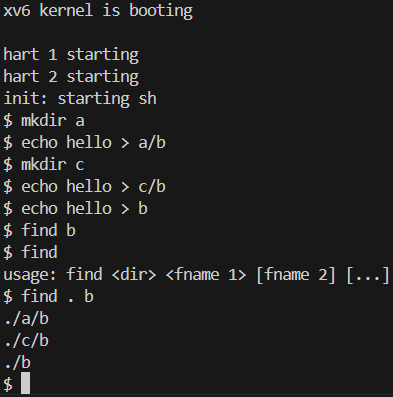
\includegraphics[width=0.5\textwidth]{figures/exec-find}
	\caption{Kết quả chạy thử \textbf{find} trên \textbf{qemu}}
\end{figure}
\begin{figure}[htp!]
	\centering
	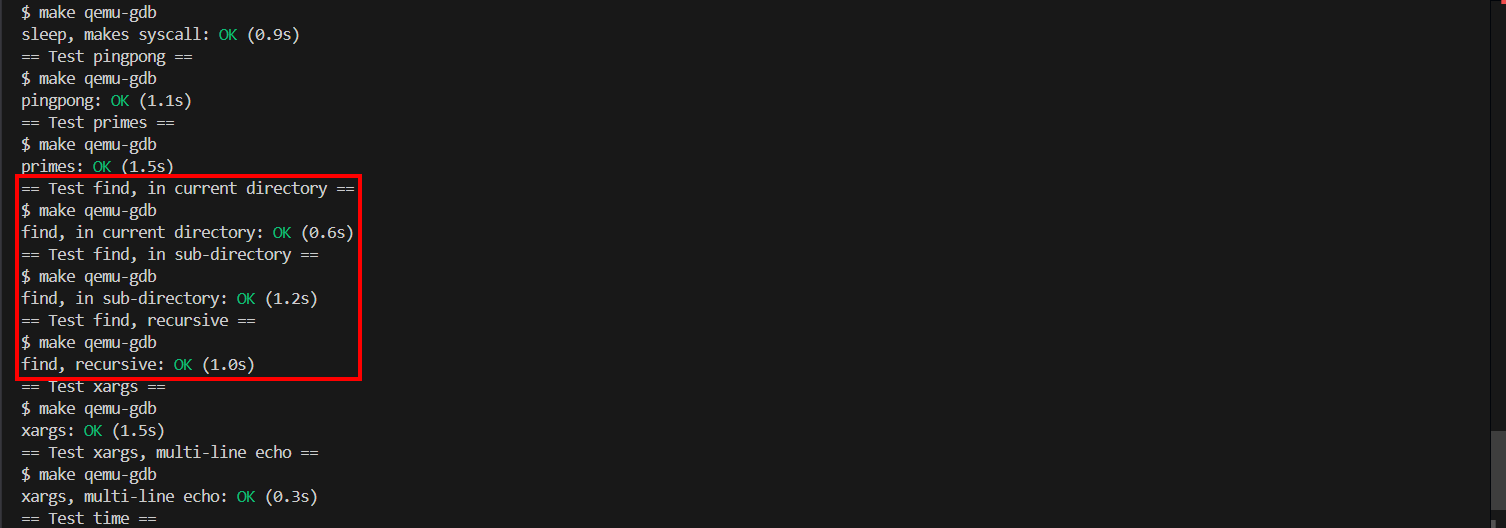
\includegraphics[width=0.9\textwidth]{figures/find-test}
	\caption{Kết quả kiểm thử \textbf{find} bằng công cụ chấm bài \textbf{grade} của MIT}
\end{figure}
  \subsection{Lệnh xargs}
\underline{\textbf{Chức năng của lệnh:}} Lệnh \verb|xargs <cmd> [args]| được dùng để thực thi lệnh được nhập từ đầu vào tiêu chuẩn bằng cách chuyển các chuỗi ký tự đầu vào thành lệnh và các đối số tương ứng \cite{mit-xv6} \cite{xargs}.

\underline{\textbf{Thiết lập thuật toán:}} (có tham khảo qua source code ở \cite{xargscode})

Hàm \mintinline{C++}|void clear(char** x_argv, int start)| được thiết lập để xóa câu lệnh đã được thực thi trước đó (vị trí bắt đầu từ \verb|start|).
Hàm \verb|main|:
\begin{enumerate}[labelindent=1em, labelsep=0.2cm, leftmargin=1cm, wide=\parindent, topsep=0.1cm, itemsep=-1ex, partopsep=1.5ex, parsep=1.5ex]
	\item Kiểm tra cú pháp của \verb|xargs|. Lệnh sẽ báo lỗi khi người dùng nhập sai cú pháp hoặc quá nhiều cú pháp (\verb|argc| vượt quá \verb|MAXARG|).
	\item Khởi tạo chuỗi \verb|buffer| để lưu các ký tự đầu, mảng các chuỗi \verb|x_argv| để lưu các chuỗi liền mạch trong \verb|buffer| và \verb|x_argc| để lưu số lượng chuỗi trong \verb|x_argv|.
	\item Đọc các ký tự sử dụng vòng lặp \verb|while|.
	\item Phân chia tiến trình bằng hàm \verb|fork()|. Tiến trình con sẽ đảm nhiệm việc chạy chương trình lưu trong \verb|x_argv|, trong khi tiến trình cha giải phóng vùng nhớ của các chuỗi trong câu lệnh đã được thực hiện trước đó. Chương trình kết thúc khi không còn ký tự đầu vào nào nữa.
\end{enumerate}

\underline{\textbf{Khó khăn đã gặp phải:}}
\begin{itemize}[labelindent=1em, labelsep=0.2cm, leftmargin=1cm, wide=\parindent, topsep=0.1cm, itemsep=-1ex, partopsep=1.5ex, parsep=1.5ex]
	\item Hiểu đúng nguyên lý hoạt động của \verb|xargs| trên Unix.
	\item Việc đọc và lưu trữ ký tự phải được thực hiện kỹ càng để không bỏ sót các lệnh/đối số hoặc đọc sai lệnh/đối số.
\end{itemize}

Dưới đây là kết quả chạy thử trên \verb|qemu| và kiểm tra lệnh \verb|xargs| bằng chương trình kiểm thử:
\begin{figure}[htp!]
	\centering
	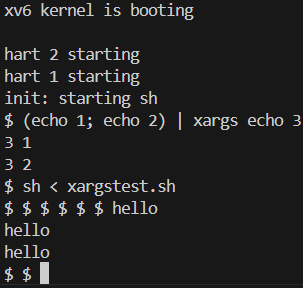
\includegraphics[width=0.5\textwidth]{figures/exec-xargs}
	\caption{Kết quả chạy thử \textbf{xargs} trên \textbf{qemu}}
\end{figure}
\begin{figure}[htp!]
	\centering
	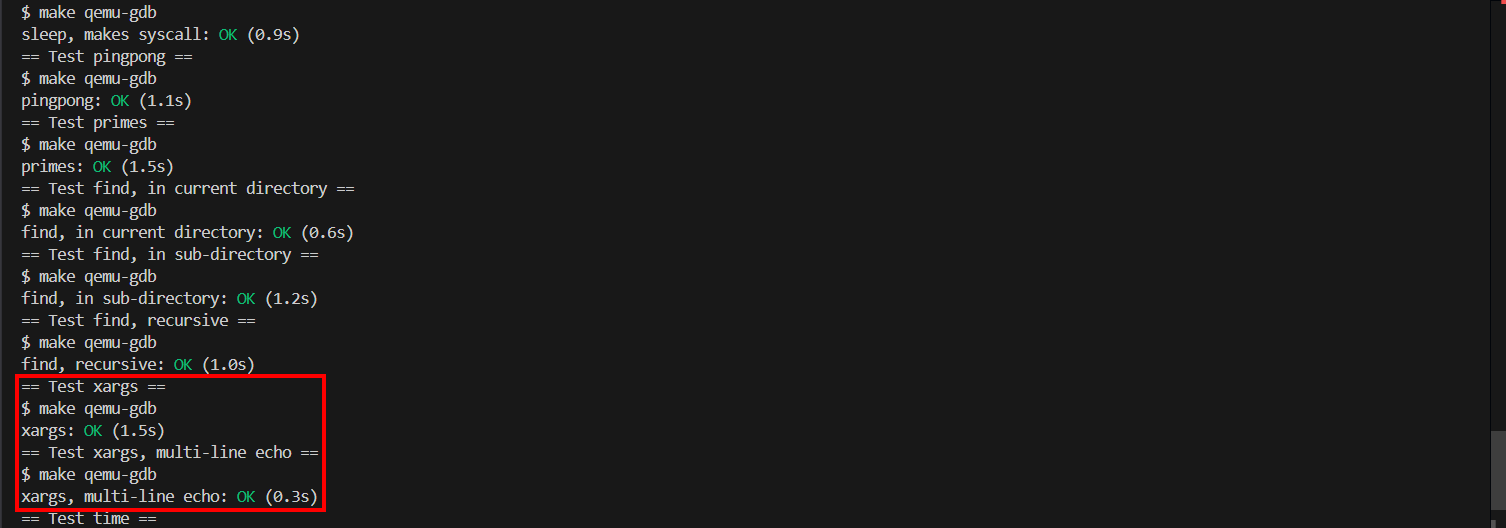
\includegraphics[width=0.9\textwidth]{figures/xargs-test}
	\caption{Kết quả kiểm thử \textbf{xargs} bằng công cụ chấm bài \textbf{grade} của MIT}
\end{figure}
  
  \newpage
  \section*{Tài liệu tham khảo}
  \addcontentsline{toc}{section}{Tài liệu tham khảo}
  \printbibliography[type = book, title = {Sách}]
  \printbibliography[type = article, title = {Bài báo}]
  \printbibliography[type = misc, title = {Internet}]
  
\end{document}